\documentclass{beamer}
\usetheme{Metropolis}  % Use the Metropolis theme
\usepackage{tikz}      % For precise positioning

\title{LUS Image Classification of Covid-19 and Pneumonia}
\author{Abhijith C}
\date{\today}

\begin{document}

\maketitle

\section{Introduction}
\begin{frame}{LUS Images}
        Lung ultrasound (LUS) images provide key diagnostic information by capturing different artifacts and structures in the lungs. Key elements in LUS images include:
\begin{itemize}
        \item \textbf{Pleural Line} – The bright, horizontal line at the top of the image, representing the lung’s surface.
        \item \textbf{A-Lines} – Repetitive horizontal artifacts indicating normal aerated lungs.
        \item \textbf{B-Lines} – Vertical, hyperechoic (bright) lines extending to the bottom, associated with lung pathologies like pneumonia and pulmonary edema.
        %\item \textbf{Consolidations} – Hypoechoic (dark) regions indicating areas of lung tissue affected by infection or inflammation.
        %\item \textbf{Pleural Effusion} – Fluid accumulation appearing as an anechoic (black) area beneath the lung.
    \end{itemize}
    
\end{frame}

\begin{frame}{LUS Images}
    \begin{columns}
        \column{0.5\textwidth}
        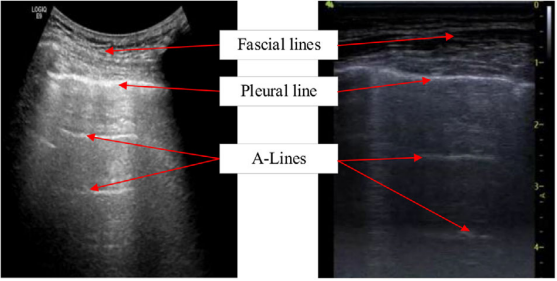
\includegraphics[width=\linewidth]{a-lines.png}
        
        \column{0.5\textwidth}
        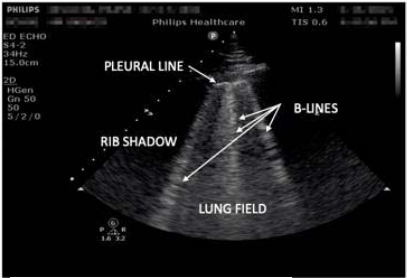
\includegraphics[width=\linewidth]{b-lines.png}
    \end{columns}
    \begin{tikzpicture}[remember picture, overlay]
        \node[anchor=south] at (current page.south) {\tiny \textbf{Image Sources: \cite{a-lines}, \cite{b-lines}}};
    \end{tikzpicture}
\end{frame}

\begin{frame}{LUS Differences: COVID-19 vs. Pneumonia}
    \centering
    \begin{tabular}{lll}
        \hline
        \textbf{Feature} & \textbf{COVID-19} & \textbf{Pneumonia} \\
        \hline
        \textbf{B-Lines} & Scattered, widespread & Localized in one area \\
        \hline
        \textbf{Pleural Line} & Thick and uneven & Mostly normal \\
        \hline
        %\textbf{Consolidations} & Less common & More frequent \\
        %\hline
        %\textbf{Pleural Effusion} & Rare & Common \\
        %\hline
        \textbf{Lung Involvement} & Both lungs (bilateral) & One lung (unilateral) \\
        \hline
    \end{tabular}
    
    \vspace{0.5cm}
    \centering
    \includegraphics[width=0.6\textwidth]{example-image}  % Replace with actual LUS image
    
    \small COVID-19 affects both lungs with scattered changes, while pneumonia is more localized.
\end{frame}


\section{Main Content}
\begin{frame}{Key Points}
    \begin{itemize}
        \item First key point
        \item Second key point
        \item Third key point
    \end{itemize}
\end{frame}

\begin{frame}{Example Chart}
    \begin{center}
        \includegraphics[width=0.8\textwidth]{example-image} % Replace with your actual image
    \end{center}
\end{frame}

\section{Conclusion}
\begin{frame}{Summary}
\end{frame}

\begin{frame}{References}
    \begin{thebibliography}{99}
        \bibitem{a-lines} Xing, Wenyu, et al. "Automatic detection of A‐line in lung ultrasound images using deep learning and image processing." Medical physics 50.1 (2023): 330-343.
	\bibitem{b-lines} Baloescu, Cristiana, et al. "Automated lung ultrasound B-line assessment using a deep learning algorithm." IEEE Transactions on Ultrasonics, Ferroelectrics, and Frequency Control 67.11 (2020): 2312-2320.
    \end{thebibliography}
\end{frame}

\end{document}
